\documentclass[12pt]{article}

\usepackage{fullpage}
\usepackage{amssymb}
\usepackage{amsthm}
\usepackage{amsmath}
\usepackage{booktabs}
\usepackage{graphicx}
\usepackage{natbib}
\usepackage[multiple]{footmisc}
\usepackage{url}
\usepackage{color,soul}
\usepackage{multirow}
\usepackage[top=1in, bottom=1.3in, left=1.5in, right=1.5in]{geometry}
\usepackage[linesnumbered,ruled]{algorithm2e}
\usepackage[labelformat=simple]{subcaption}
\renewcommand\thesubfigure{(\alph{subfigure})}

\usepackage{tikz}
\usetikzlibrary{arrows,shapes,calc,positioning}

\newcommand{\dif}{\operatorname{d}}
\newcommand{\var}{\operatorname{Var}}
\newcommand{\bfx}[1]{{\bf #1}}
\newcommand{\cov}{\operatorname{Cov}}


\title{Data and Systems}

\author{Guojun Gan\thanks{Department of Mathematics, University of Connecticut, 341 Mansfield Road, Storrs, CT, 06268-1009, USA. Email: \texttt{guojun.gan@uconn.edu}.}}

\begin{document}

\maketitle

This chapter covers the learning areas on data and systems outlined in the IAA ( International Actuarial Association) Education Syllabus published in September 2015.

\section{Data}

% 7.1.3 - 7.1.6 data source, structure, storage, quality, preprocessing tools  inmon2014
% 7.4.1 - 7.4.3 ethical (miles2014), governance, risks
%
\subsection{Data Types and Sources}

In terms of how data are collected, data can be divided into two types \citep{hox2005data}: primary data and secondary data. Primary data are original data that are collected for a specific research problem. Secondary data are data originally collected for a different purpose and reused for another research problem. A major advantage of using primary data is that the theoretical constructs, the research design, and the data collection strategy can be tailored to the underlying research question to ensure that the data collected indeed help to solve the problem. A disadvantage of using primary data is that data collection can be costly and time-consuming. Using secondary data has the advantage of lower cost and faster access to relevant information. However, using secondary data may not be optimal for the research question under consideration.   

In terms of the degree of organization of the data, data can be also divided into two types \citep{inmon2014,leary2013bigdata,hashem2015bigdata,abdullah2013data,pries2015}: structured data and unstructured data. Structured data have a predictable and regularly occurring format. In contrast, unstructured data are unpredictable and have no structure that is recognizable to a computer. Structured data consists of records, attributes, keys, and indices and are typically managed by a database management system (DBMS) such as IBM DB2, Oracle, MySQL, and Microsoft SQL Server. As a result, most units of structured data can be located quickly and easily. Unstructured data have many different forms and variations. One common form of unstructured data is text. Accessing unstructured data is clumsy. To find a given unit of data in a long text, for example, sequentially search is usually performed. 

In terms of how the data are measured, data can be classified as qualitative or quantitative. Qualitative data is data about qualities, which cannot be actually measured. As a result, qualitative data is extremely varied in nature and includes interviews, documents, and artifacts \citep{miles2014}. Quantitative data is data about quantities, which can be measured numerically with numbers. In terms of the level of measurement, quantitative data can be further classified as nominal, ordinal,  interval, or ratio \citep{gan2011}. Nominal data, also called categorical data, are discrete data without a natural ordering. Ordinal data are discrete data with a natural order. Interval data are continuous data with a specific order and equal intervals. Ratio data are interval data with a natural zero. 

There exist a number of data sources. First, data can be obtained from university-based researchers who collect primary data. Second, data can be obtained from organizations that are set up for the purpose of releasing secondary data for general research community. Third, data can be obtained from national and regional statistical institutes that collect data. Finally, companies have corporate data that can be obtained for research purpose.

While it might be difficult to obtain data to address a specific research problem or answer a business question, it is relatively easy to obtain data to test a model or an algorithm for data analysis. In nowadays, readers can obtain datasets from the Internet easily. The following is a list of some websites to obtain real-world data:
\begin{description}
\item[UCI Machine Learning Repository] This website (url: \url{http://archive.ics.uci.edu/ml/index.php}) maintains more than 400 datasets that can be used to test machine learning algorithms.
\item[Kaggle] The Kaggle website (url: \url{https://www.kaggle.com/}) include real-world datasets used for data science competition. Readers can download data from Kaggle by registering an account.
\item[DrivenData] DrivenData aims at bringing cutting-edge practices in data science to solve some of the world's biggest social challenges. In its website (url: \url{https://www.drivendata.org/}), readers can participate data science competitions and download datasets.
\item[Analytics Vidhya] This website (url: \url{https://datahack.analyticsvidhya.com/contest/all/}) allows you to participate and download datasets from practice problems and hackathon problems. 
\item[KDD Cup] KDD Cup is the annual Data Mining and Knowledge Discovery competition organized by ACM Special Interest Group on Knowledge Discovery and Data Mining. This website (url: \url{http://www.kdd.org/kdd-cup}) contains the datasets used in past KDD Cup competitions since 1997.
\item[U.S. Government's open data] This website (url: \url{https://www.data.gov/}) contains about 200,000 datasets covering a wide range of areas including climate, education, energy, and finance.
\item[AWS Public Datasets] In this website (url: \url{https://aws.amazon.com/datasets/}), Amazon provides a centralized repository of public datasets, including some huge datasets.
\end{description}


\subsection{Data Structures and Storage}

As mentioned in the previous subsection, there are structured data as well as unstructured data. Structured data are highly organized data and usually have the following tabular format:
\begin{center}
\begin{tabular}{lllll}
\toprule
 & $V_1$ & $V_2$ & $\cdots$ & $V_d$ \\
\midrule
$\bfx{x}_1$ & $x_{11}$ & $x_{12}$ & $\cdots$ & $x_{1d}$ \\
$\bfx{x}_2$ & $x_{21}$ & $x_{22}$ & $\cdots$ & $x_{2d}$ \\
$\vdots$ & $\vdots$ & $\vdots$ & $\cdots$ & $\vdots$ \\
$\bfx{x}_n$ & $x_{n1}$ & $x_{n2}$ & $\cdots$ & $x_{nd}$ \\
\bottomrule
\end{tabular}
\end{center}
In other words, structured data can be organized into a table consists of rows and columns. Typically, each row represents a record and each column represents an attribute. A table can be decomposed into several tables that can be stored in a relational database such as the Microsoft SQL Server. The SQL (Structured Query Language) can be used to access and modify the data easily and efficiently.

Unstructured data do not follow a regular format \citep{abdullah2013data}. Examples of unstructured data include documents, videos, and audio files. Most of the data we encounter are unstructured data. In fact, the term ``big data'' was coined to reflect this fact. Traditional relational databases cannot meet the challenges on the varieties and scales brought by massive unstructured data nowadays. NoSQL databases have been used to store massive unstructured data. 

There are three main NoSQL databases \citep{chen2014b}: key-value databases, column-oriented databases, and document-oriented databases. Key-value databases use a simple data model and store data according to key-values. Modern key-value databases have higher expandability and smaller query response time than relational databases. Examples of key-value databases include Dynamo used by Amazon and Voldemort used by LinkedIn. Column-oriented databases store and process data according to columns rather than rows. The columns and rows are segmented in multiple nodes to achieve expandability. Examples of column-oriented databases include BigTable developed by Google and Cassandra developed by FaceBook. Document databases are designed to support more complex data forms than those stored in key-value databases. Examples of document databases include MongoDB, SimpleDB, and CouchDB. MongoDB is an open-source document-oriented database that stores documents as binary objects. SimpleDB is a distributed NoSQL database used by Amazon. CouchDB is an another open-source document-oriented database. 

\subsection{Data Quality}

Accurate data are essential to useful data analysis. The lack of accurate data may lead to significant costs to organizations in areas such as correction activities, lost customers, missed opportunities, and incorrect decisions \citep{olson2003}.

Data has quality if it satisfies its intended use, that is, the data is accurate, timely, relevant, complete, understood, and trusted \citep{olson2003}. As a result, we first need to know the specification of the intended uses and then judge the suitability for those uses in order to assess the quality of the data. Unintended uses of data can arise from a variety of reasons and lead to serious problems. 

Accuracy is the single most important component of high-quality data. Accurate data have the following properties \citep{olson2003}:
\begin{itemize}
\item The data elements are not missing and have  valid values.
\item The values of the data elements are in the right ranges and have the right representations.
\end{itemize}
Inaccurate data arise from different sources. In particular, the following areas are common areas where inaccurate data occur:
\begin{itemize}
\item Initial data entry. Mistakes (including deliberate errors) and system errors can occur during the initial data entry. Flawed data entry processes can result in inaccurate data.
\item Data decay. Data decay, also known as data degradation, refers to the gradual corruption of computer data due to an accumulation of non-critical failures in a storage device.
\item Data moving and restructuring. Inaccurate data can also arise from data extracting, cleaning, transforming, loading, or integrating.
\item Data using. Faulty reporting and lack of understanding can lead to inaccurate data.
\end{itemize}

Reverification and analysis are two approaches to find inaccurate data elements. To ensure that the data elements are 100\% accurate, we must use reverification. However, reverification can be time-consuming and may not be possible for some data. Analytical techniques can also be used to identify inaccurate data elements. There are five types of analysis that can be used to  identify inaccurate data \citep{olson2003}: data element analysis, structural analysis, value correlation, aggregation correlation, and value inspection

Companies can create a data quality assurance program to create high-quality databases. For more information about data quality issues management and data profiling techniques, readers are referred to \citep{olson2003}.

\subsection{Data Cleaning}

Raw data usually need to be cleaned before useful analysis can be conducted. In particular, the following areas need attention when preparing data for analysis \citep{janert2010}:
\begin{description}
\item[Missing values] It is common to have missing values in raw data. Depending on the situations, we can discard the record, discard the variable, or impute the missing values.
\item[Outliers] Raw data may contain unusual data points such as outliers. We need to handle outliers carefully. We cannot just remove outliers without knowing the reason for their existence. Sometimes the outliers are caused by clerical errors. Sometimes outliers are the effect we are looking for.
\item[Junk] Raw data may contain junks such as nonprintable characters. Junks are typically rare and not easy to get noticed. However, junks can cause serious problems in downstream applications.
\item[Format] Raw data may be formated in a way that is inconvenient for subsequent analysis. For example, components of a record may be split into multiple lines in a text file. In such cases, lines corresponding to a single record should be merged before loading to a data analysis software such as R.
\item[Duplicate records] Raw data may contain duplicate records. Duplicate records should be recognized and removed. This task may not be trivial depending on what you consider ``duplicate.''
\item[Merging datasets] Raw data may come from different sources. In such cases, we need to merge the data from different sources to ensure compatibility.
\end{description}

For more information about how to handle data in R, readers are referred to \citep{forte2015} and \citep{buttrey2017}.

\section{Data Analysis Preliminary}

% aims 7.1.1  stages 7.1.2
% 7.5.1 visualization reporting
% 7.5.2 reproducible mailund2017


Data analysis involves inspecting, cleansing, transforming, and modeling data to discover useful information to suggest conclusions and make decisions. Data analysis has a long history. In 1962, statistician John Tukey defined data analysis as \citep{tukey1962data}: 
\begin{quote}
procedures for analyzing data,  techniques for interpreting the results of such procedures, ways of planning the  gathering of data to make its analysis easier, more precise or more accurate, and  all the machinery and results of (mathematical) statistics which apply to analyzing data.
\end{quote}
Recently, Judd and coauthors defined data analysis as the following equation \citep{judd2017}:
\begin{equation}\label{eq:judd}
\hbox{Data} = \hbox{Model} + \hbox{Error},
\end{equation}
where Data represents a set of basic scores or observations to be analyzed, Model is a compact representation of the data, and Error is simply the amount the model fails to represent accurately. Using the above equation for data analysis, an analyst must resolve the following two conflicting goals:
\begin{itemize}
\item to add more parameters to the model so that the model represents the data better.
\item to remove parameters from the model so that the model is simple and parsimonious.
\end{itemize}

In this section, we give a high-level introduction to data analysis, including different types of methods.

\subsection{Data Analysis Process}\label{sec:process}

Data analysis is part of an overall study. For example, Figure \ref{fig:study} shows the process of a typical study in behavioral and social sciences as described in \citep{albers2017}. The data analysis part consists of the following steps:
\begin{description}
\item[Exploratory analysis] The purpose of this step is to get a feel of the relationships with the data and figure out what type of analysis for the data makes sense.
\item[Statistical analysis] This step performs statistical analysis such as determining statistical significance and effect size. 
\item[Make sense of the results] This step interprets the statistical results in the context of the overall study.
\item[Determine implications] This step interprets the data by connecting it to the study goals and the larger field of this study.
\end{description}
The goal of the data analysis as described above focuses on explaining some phenomenon (See Section \ref{sec:expred}). 

\begin{figure}[htbp]
\centering
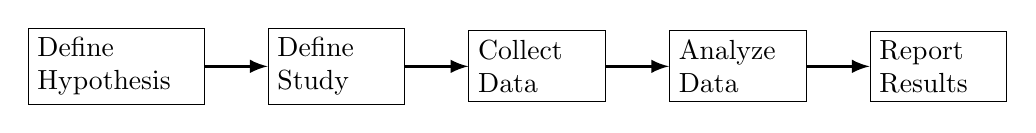
\begin{tikzpicture}[node distance=0.8cm]
\node[rectangle, draw=black, text width=2cm](s1){Define\\ Hypothesis};
\node[right =of s1, rectangle, draw=black, text width=1.5cm](s2){Define\\ Study};
\node[right=of s2, rectangle, draw=black, text width=1.5cm](s3){Collect Data};
\node[right =of s3, rectangle, draw=black, text width=1.5cm](s4){Analyze Data};
\node[right =of s4, rectangle, draw=black, text width=1.5cm](s5){Report Results};
\draw[->,>=latex,very thick] (s1)--(s2);
\draw[->,>=latex,very thick] (s2)--(s3);
\draw[->,>=latex,very thick] (s3)--(s4);
\draw[->,>=latex,very thick] (s4)--(s5);
\end{tikzpicture}
\caption{The process of a typical study in behavioral and social sciences.}\label{fig:study}
\end{figure}

\cite{shmueli2010model} described a general process for statistical modeling, which is shown in Figure \ref{fig:modeling}. Depending on the goal of the analysis, the steps differ in terms of the choice of methods, criteria, data, and information.

\begin{figure}[htbp]
\centering
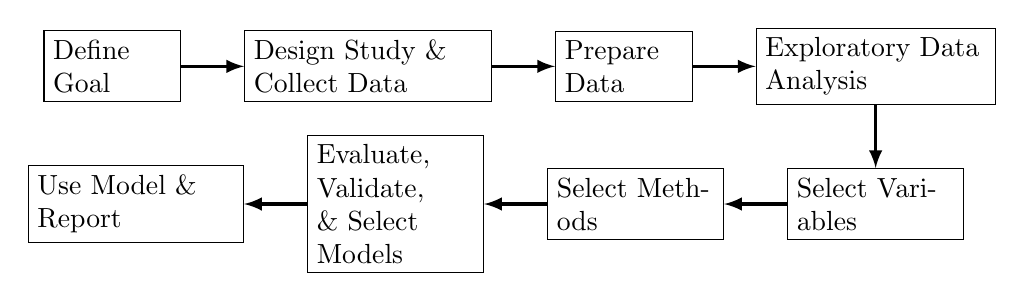
\begin{tikzpicture}[node distance=0.8cm]
\node[rectangle, draw=black, text width=1.5cm](s1){Define\\ Goal};
\node[right =of s1, rectangle, draw=black, text width=2.9cm](s2){Design Study \& \\ Collect Data};
\node[right=of s2, rectangle, draw=black, text width=1.5cm](s3){Prepare Data};
\node[right =of s3, rectangle, draw=black, text width=2.8cm](s4){Exploratory Data Analysis};
\node[below =of s4, rectangle, draw=black, text width=2cm](s5){Select Variables};
\node[left =of s5, rectangle, draw=black, text width=2cm](s6){Select Methods};
\node[left =of s6, rectangle, draw=black, text width=2cm](s7){Evaluate, Validate,\\ \& Select Models};
\node[left =of s7, rectangle, draw=black, text width=2.5cm](s8){Use Model \& \\ Report};
\draw[->,>=latex,very thick] (s1)--(s2);
\draw[->,>=latex,very thick] (s2)--(s3);
\draw[->,>=latex,very thick] (s3)--(s4);
\draw[->,>=latex,very thick] (s4)--(s5);
\draw[->,>=latex,very thick] (s5)--(s6);
\draw[->,>=latex,very thick] (s6)--(s7);
\draw[->,>=latex,very thick] (s7)--(s8);
\end{tikzpicture}
\caption{The process of statistical modeling.}\label{fig:modeling}
\end{figure}



\subsection{Exploratory versus Confirmatory}
There are two phases of data analysis \citep{good1983data}: exploratory data analysis (EDA) and confirmatory data analysis (CDA). Table \ref{tbl:edacda} summarizes some differences between EDA and CDA. EDA is usually applied to observational data with the goal of looking for patterns and formulating hypotheses. In contrast, CDA 
is often applied to experimental data (i.e., data obtained by means of a formal design of experiments) with the goal of quantifying the extent to which discrepancies between the model and the data could be expected to occur by chance \citep{gelman2004eda}. 

\begin{table}[htbp]
\centering
\caption{Comparison of exploratory data analysis and confirmatory data analysis.}\label{tbl:edacda}
\begin{tabular}{lll}
\toprule
 & \textbf{EDA} & \textbf{CDA} \\
\midrule
Data & Observational data & Experimental data\\[3mm]
Goal & Pattern recognition,  & Hypothesis testing,  \\
& formulate hypotheses & estimation, prediction \\[3mm]
Techniques & Descriptive statistics, & Traditional statistical tools of \\
& visualization, clustering & inference, significance, and\\
& & confidence \\
\bottomrule
\end{tabular}
\end{table}

Techniques for EDA include descriptive statistics (e.g., mean, median, standard deviation, quantiles), distributions, histograms, correlation analysis, dimension reduction, and cluster analysis. Techniques for CDA include the traditional statistical tools of inference, significance, and confidence.

\subsection{Supervised versus Unsupervised}

Methods for data analysis can be divided into two types \citep{abbott2014,igual2017}: supervised learning methods and unsupervised learning methods. Supervised learning methods work with labeled data, which include a target variable. Mathematically, supervised learning methods try to approximate the following function:
\[
Y = f(X_1, X_2, \ldots, X_p),
\]
where $Y$ is a target variable and $X_1$, $X_2$, $\ldots$, $X_p$ are explanatory variables.  Other terms are also used to mean a target variable. Table \ref{tbl:lmnames} gives a list of common names for different types of variables \citep{frees2009}. When the target variable is a categorical variable, supervised learning methods are called classification methods. When the target variable is continuous, supervised learning methods are called regression methods.

\begin{table}[htb]
\centering
\begin{tabular}{ll}
\toprule
\textbf{Target Variable}  &  \textbf{Explanatory Variable}\\
\midrule
Dependent variable & Independent variable\\
Response & Treatment \\
Output & Input \\
Endogenous variable & Exogenous variable \\
Predicted variable & Predictor variable \\
Regressand & Regressor \\
\bottomrule
\end{tabular}
\caption{Common names of different variables.}\label{tbl:lmnames}
\end{table}


Unsupervised learning methods work with unlabeled data, which include explanatory variables only. In other words, unsupervised learning methods do not use target variables. As a result, unsupervised learning methods are also called descriptive modeling methods.

\subsection{Parametric versus Nonparametric}

Methods for data analysis can be parametric or nonparametric \citep{abbott2014}. Parametric methods assume that the data follow a certain distribution. Nonparametric methods do not assume distributions for the data and therefore are called distribution-free methods.

Parametric methods have the advantage that if the distribution of the data is known, properties of the data and properties of the method (e.g., errors, convergence, coefficients) can be derived. A disadvantage of parametric methods is that analysts need to spend considerable time on figuring out the distribution. For example, analysts may try different transformation methods to transform the data so that it follows a certain distribution.

Since nonparametric methods make fewer assumptions, nonparametric methods have the advantage that they are more flexible, more robust, and applicable to non-quantitative data. However, a drawback of nonparametric methods is that the conclusions drawn from nonparametric methods are not as powerful as those drawn from parametric methods.  

\subsection{Explanation versus Prediction}\label{sec:expred}

There are two goals in data analysis \citep{breiman2001modeling,shmueli2010model}: explanation and prediction. In some scientific areas such as economics, psychology, and environmental science, the focus of data analysis is to explain the causal relationships between the input variables and the response variable. In other scientific areas such as natural language processing and bioinformatics, the focus of data analysis is to predict what the responses are going to be given the input variables.

\cite{shmueli2010model} discussed in detail the distinction between explanatory modeling and predictive modeling, which reflect the process of using data and methods for explaining or predicting, respectively. Explanatory modeling is commonly used for theory building and testing. However, predictive modeling is rarely used in many scientific fields as a tool for developing theory.  

Explanatory modeling is typically done as follows:
\begin{itemize}
\item State the prevailing theory.
\item State causal hypotheses, which are given in terms of theoretical constructs rather than measurable variables. A causal diagram is usually included to illustrate the hypothesized causal relationship between the theoretical constructs.
\item Operationalize constructs. In this step, previous literature and theoretical justification are used to build a bridge between theoretical constructs and observable measurements.
\item Collect data and build models alongside the statistical hypotheses, which are operationalized from the research hypotheses. 
\item Reach research conclusions and recommend policy. The statistical conclusions are converted into research conclusions. Policy recommendations are often accompanied.
\end{itemize}

\cite{shmueli2010model} defined predictive modeling as the process of applying a statistical model or data mining algorithm to data for the purpose of predicting new or future observations. Predictions include point predictions, interval predictions, regions, distributions, and rankings of new observations. Predictive model can be any method that produces predictions. 

 

\subsection{Data Modeling versus Algorithmic Modeling}

\cite{breiman2001modeling} discussed two cultures in the use of statistical modeling to reach conclusions from data: the data modeling culture and the algorithmic modeling culture. In the data modeling culture, the data are assumed to be generated by a given stochastic data model. In the algorithmic modeling culture, the data mechanism is treated as unknown and algorithmic models are used.

Data modeling gives the statistics field many successes in analyzing data and getting information about the data mechanisms. However, \cite{breiman2001modeling} argued that the focus  on data models in the statistical community has led to some side effects such as
\begin{itemize}
\item Produced irrelevant theory and questionable scientific conclusions.
\item Kept statisticians from using algorithmic models that might be more suitable.
\item Restricted the ability of statisticians to deal with a wide range of problems.
\end{itemize}

Algorithmic modeling was used by industrial statisticians long time ago. However, the development of algorithmic methods was taken up by a community outside statistics \citep{breiman2001modeling}. The goal of algorithmic modeling is predictive accuracy. For some complex prediction problems, data models are not suitable. These prediction problems include speech recognition, image recognition, handwriting recognition, nonlinear time series prediction, and financial market prediction. The theory in algorithmic modeling focuses on the properties of algorithms, such as convergence and predictive accuracy. 

\subsection{Big Data Analysis}

Unlike traditional data analysis, big data analysis employs additional methods and tools that can extract information rapidly from massive data. In particular, big data analysis uses the following processing methods \citep{chen2014b}:
\begin{description}
\item[Bloom filter] A bloom filter is a space-efficient probabilistic data structure that is used to determine whether an element belongs to a set. It has the advantages of high space efficiency and high query speed. A drawback of using bloom filter is that there is a certain misrecognition rate.
\item[Hashing] Hashing is a method that transforms data into  fixed-length numerical values through a hash function. It has the advantages of rapid reading and writing. However, sound hash functions are difficult to find. 
\item[Indexing] Indexing refers to a process of partitioning data in order to speed up reading. Hashing is a special case of indexing.
\item[Tries] A trie,  also called digital tree, is a method to improve query efficiency by using common prefixes of character strings to reduce comparison on character strings to the greatest extent.
\item[Parallel computing] Parallel computing uses multiple computing resources to complete a computation task. Parallel computing tools include MPI (Message Passing Interface), MapReduce, and Dryad.
\end{description}

Big data analysis can be conducted in the following levels \citep{chen2014b}: memory-level, business intelligence (BI) level, and massive level. Memory-level analysis is conducted when the data can be loaded to the memory of a cluster of computers. Current hardware can handle hundreds of gigabytes (GB) of data in memory. BI level analysis can be conducted when the data surpass the memory level. It is common for BI level analysis products to support data over terabytes (TB). Massive level analysis is conducted when the data surpass the capabilities of products for BI level analysis. Usually Hadoop and MapReduce are used in massive level analysis. 

\subsection{Reproducible Analysis}

As mentioned in Section \ref{sec:process}, a typical data analysis workflow includes collecting data, analyzing data, and reporting results. The data collected are saved in a database or files. The data are then analyzed by one or more scripts, which may save some intermediate results or always work on the raw data. Finally a report is produced to describe the results, which include relevant plots, tables, and summaries of the data. The workflow may subject to the following potential issues \citep[Chapter 2]{mailund2017}:
\begin{itemize}
\item The data are separated from the analysis scripts.
\item The documentation of the analysis is separated from the analysis itself. 
\end{itemize} 

If the analysis is done on the raw data with a single script, then the first issue is not a major problem. If the analysis consists of multiple scripts and a script saves intermediate results that are read by the next script, then the scripts describe a workflow of data analysis. To reproduce an analysis, the scripts have to be executed in the right order. The workflow may cause major problems if the order of the scripts is not documented or the documentation is not updated or lost. One way to address the first issue is to write the scripts so that any part of the workflow can be run completely automatically at any time.

If the documentation of the analysis is synchronized with the analysis, then the second issue is not a major problem. However, the documentation may become completely useless if the scripts are changed but the documentation is not updated.

Literate programming is an approach to address the two issues mentioned above. In literate programming, the documentation of a program and the code of the program are written together. To do literate programming in R, one way is to use the R Markdown and the \texttt{knitr} package.

\subsection{Ethical Issues}

Analysts may face ethical issues and dilemmas during the data analysis process. In some fields, for example, ethical issues and dilemmas include participant consent, benefits, risk, confidentiality, and data ownership \citep{miles2014}. For data analysis in actuarial science and insurance in particular, we face the following ethical matters and issues \citep{miles2014}:
\begin{description}
\item[Worthness of the project] Is the project worth doing? Will the project contribute in some significant way to a domain broader than my career? If a project is only opportunistic and does not have a larger significance, then it might be pursued with less care. The result may be looked good but not right.
\item[Competence] Do I or the whole team have the expertise to carry out the project? Incompetence may lead to weakness in the analytics such as collecting large amounts of data poorly and drawing superficial conclusions.
\item[Benefits, costs, and reciprocity] Will each stakeholder gain from the project? Are the benefit and the cost equitable? A project will likely to fail if the benefit and the cost for a stakeholder do not match.
\item[Privacy and confidentiality] How do we make sure that the information is kept confidentially? Where raw data and analysis results are stored and how will have access to them should be documented in explicit confidentiality agreements. 

\end{description}



\section{Data Analysis Techniques}

% 7.2.1 - 7.2.3 exploratory, summarize, pca
% 7.3.1 - 7.3.3 machine learning, problems solved by ml, techniques
% statistics, machine learning, pattern recognition, data mining, predictive analytics, business intelligence, artificial intelligence

Techniques for data analysis are drawn from different but overlapping fields such as statistics, machine learning, pattern recognition, and data mining. Statistics is a field that addresses reliable ways of gathering data and making inferences based on them \citep{bandyo2011,bluman2012}. The term machine learning was coined by Samuel in 1959 \citep{samuel1959ml}. Originally, machine learning refers to the field of study where computers have the ability to learn without being explicitly programmed. Nowadays, machine learning has evolved to the broad field of study where computational methods use experience (i.e., the past information available for analysis) to improve performance or to make accurate predictions \citep{bishop2007,clarke2009,mohri2012,kubat2017}. There are four types of machine learning algorithms (See Table \ref{tbl:mlalg}) depending on the type of the data and the type of the learning tasks.


\begin{table}[htbp]
  \centering
  \caption{Types of machine learning algorithms.}
  \label{tbl:mlalg}%
    \begin{tabular}{rll}
    \toprule
          & \textbf{Supervised} & \textbf{Unsupervised} \\
    \midrule
    \textbf{Discrete Label} & Classification & Clustering \\
    \textbf{Continuous Label} & Regression & Dimension reduction \\
    \bottomrule
    \end{tabular}%
\end{table}%

Originating in engineering, pattern recognition is a field that is closely related to machine learning, which grew out of computer science. In fact, pattern recognition and machine learning can be considered to be two facets of the same field \citep{bishop2007}. Data mining is a field that concerns collecting, cleaning, processing, analyzing, and gaining useful insights from data \citep{aggarwal2015}.


\subsection{Exploratory Techniques}

Exploratory data analysis techniques include descriptive statistics as well as many unsupervised learning techniques such as data clustering and principal component analysis.

\subsubsection{Descriptive Statistics}

In the mass noun sense, descriptive statistics is an area of statistics that concerns the collection, organization, summarization, and presentation of data \citep{bluman2012}. In the count noun sense, descriptive statistics are summary statistics that quantitatively describe or summarize data.

\begin{table}[htbp]
\centering
\caption{Some commonly used descriptive statistics.}\label{tbl:desstat}
\begin{tabular}{ll}
\toprule
 & \textbf{Descriptive Statistics} \\
\midrule
Measures of central tendency & Mean, median, mode, midrange\\
Measures of variation & Range, variance, standard deviation \\
Measures of position & Quantile \\
\bottomrule
\end{tabular}
\end{table}

Table \ref{tbl:desstat} lists some commonly used descriptive statistics. In R, we can use the function \texttt{summary} to calculate some of the descriptive statistics. For numeric data, we can visualize the descriptive statistics using a boxplot.

In addition to these quantitative descriptive statistics, we can also qualitatively describe shapes of the distributions \citep{bluman2012}. For example, we can say that a distribution is positively skewed, symmetric, or negatively skewed. To visualize the distribution of a variable, we can draw a histogram.

\subsubsection{Principal Component Analysis}

Principal component analysis (PCA) is a statistical procedure that transforms a dataset described by possibly correlated variables into a dataset described by linearly uncorrelated variables, which are called principal components and are ordered according to their variances. PCA is a technique for dimension reduction. If the original variables are highly correlated, then the first few principal components can account for most of the variation of the original data.  

To describe PCA, let $X_1,X_2,\ldots,X_d$ be a set of variables. The first principal component is defined to be the normalized linear combination of the variables that has the largest variance, that is, the first principal component is defined as
\begin{equation}\label{eq:pca-z1}
Z_1=w_{11} X_1 + w_{12} X_2 + \cdots + w_{1d} X_d,
\end{equation}
where $\bfx{w}_1=(w_{11}, w_{12}, \ldots, w_{1d})'$ is a vector of loadings such that $\var{(Z_1)}$ is maximized subject to the following constraint:
\begin{equation}
\bfx{w}_1'\bfx{w}_1 = \sum_{j=1}^d w_{1j}^2 = 1.
\end{equation}

For $i=2,3,\ldots,d$, the $i$th principal component is defined as
\begin{equation}\label{eq:pca-zi}
Z_i=w_{i1} X_1 + w_{i2} X_2 + \cdots + w_{id} X_d,
\end{equation}
where $\bfx{w}_i=(w_{i1}, w_{i2}, \ldots, w_{id})'$ is a vector of loadings such that $\var{(Z_i)}$ is maximized subject to the following constraints:
\begin{subequations}
\begin{equation}
\bfx{w}_i'\bfx{w}_i=\sum_{j=1}^d w_{ij}^2 = 1,
\end{equation}
\begin{equation}
\cov{(Z_i, Z_j)} = 0,\quad j=1,2,\ldots,i-1.
\end{equation}
\end{subequations}

The principal components of the variables are related to the eigenvectors and eigenvectors of the covariance matrix of the variables. For $i=1,2,\ldots,d$, let $(\lambda_i, \bfx{e}_i)$ be the $i$th eigenvalue-eigenvector pair of the covariance matrix ${\Sigma}$ such that $\lambda_1\ge \lambda_2\ge \ldots\ge \lambda_d\ge 0$ and the eigenvectors are normalized. Then the $i$th principal component is given by
\begin{equation}\label{eq:pca-pci}
Z_{i} = \bfx{e}_i' \bfx{X} =\sum_{j=1}^d e_{ij} X_j,
\end{equation} 
where $\bfx{X}=(X_1,X_2,\ldots,X_d)'$. It can be shown that $\var{(Z_i)} = \lambda_i$. As a result, the proportion of variance explained by the $i$th principal component is calculated as
\begin{equation}\label{eq:pca-proportion}
\dfrac{\var{(Z_i)}}{ \sum_{j=1}^{d} \var{(Z_j)}} = \dfrac{\lambda_i}{\lambda_1+\lambda_2+\cdots+\lambda_d}. 
\end{equation}

For more information about PCA, readers are referred to \citep{mirkin2011}.

\subsubsection{Cluster Analysis}

Cluster analysis (aka data clustering) refers to the process of dividing a dataset into homogeneous groups or clusters such that points in the same cluster are similar and points from different clusters are quite distinct \citep{gan2007,gan2011}. Data clustering is one of the most popular tools for exploratory data analysis and has found applications in many scientific areas. 

During the past several decades, many clustering algorithms have been proposed. Among these clustering algorithms, the $k$-means algorithm is perhaps the most well-known algorithm due to its simplicity. To describe the $k$-means algorithm, let $X=\{\bfx{x}_1,\bfx{x}_2,\ldots,\bfx{x}_n\}$ be a dataset containing $n$ points, each of which is described by $d$ numerical features. Given a desired number of clusters $k$, the $k$-means algorithm aims at minimizing the following objective function:
\begin{equation}\label{eq:kmeanobj}
P(U,Z) = \sum_{l=1}^k\sum_{i=1}^n u_{il} \Vert \bfx{x}_i-\bfx{z}_l\Vert^2,
\end{equation}
where $U=(u_{il})_{n\times k}$ is an $n\times k$ partition matrix, $Z=\{\bfx{z}_1,\bfx{z}_2,\ldots,\bfx{z}_k\}$ is a set of cluster centers, and $\Vert\cdot\Vert$ is the $L^2$ norm or Euclidean distance. The partition matrix $U$ satisfies the following conditions:
\begin{subequations}\label{eq:ucond}
	\begin{equation}\label{eq:uconda}
	u_{il}\in \{0,1\},\quad i=1,2,\ldots,n,\:l=1,2,\ldots,k,
	\end{equation}
	\begin{equation}\label{eq:ucondb}
	\sum_{l=1}^k u_{il}=1,\quad i=1,2,\ldots,n.
	\end{equation}
\end{subequations}

The $k$-means algorithm employs an iterative procedure to minimize the objective function. It repeatedly updates the partition matrix $U$ and the cluster centers $Z$ alternately until some stop criterion is met. When the cluster centers $Z$ are fixed, the partition matrix $U$ is updated as follows:
\begin{equation}\label{eq:kmean-U}
u_{il}=\left\{
\begin{array}{ll}
1, & \hbox{if $\Vert \bfx{x}_i - \bfx{z}_l\Vert = \min_{1\le j\le k} \Vert \bfx{x}_i - \bfx{z}_j\Vert$;}\\
0, & \hbox{if otherwise},
\end{array}
\right.
\end{equation}
When the partition matrix $U$ is fixed, the cluster centers are updated as follows:
\begin{equation}\label{eq:kmean-Z}
z_{lj} = \dfrac{\sum_{i=1}^n u_{il} x_{ij} } { \sum_{i=1}^n u_{il}},\quad l=1,2,\ldots,k,\: j=1,2,\ldots,d,
\end{equation}
where $z_{lj}$ is the $j$th component of $\bfx{z}_l$ and $x_{ij}$ is the $j$th component of $\bfx{x}_i$.

For more information about $k$-means, readers are referred to \citep{gan2007} and \citep{mirkin2011}.

\subsection{Confirmatory Techniques}

Confirmatory data analysis techniques include the traditional statistical tools of inference, significance, and confidence.

\subsubsection{Linear Models}

Linear models, also called linear regression models, aim at using a linear function to approximate the relationship between the dependent variable and independent variables. A linear regression model is called a simple linear regression model if there is only one independent variable. When more than one independent variables are involved, a linear regression model is called a multiple linear regression model.

Let $X$ and $Y$ denote the independent and the dependent variables, respectively. For $i=1,2,\ldots,n$, let $(x_i, y_i)$ be the observed values of $(X,Y)$ in the $i$th case.  Then the simple linear regression model is specified as follows \citep{frees2009}:
\begin{equation}\label{eq:basiclm-model}
y_i  = \beta_0 + \beta_1 x_i + \epsilon_i,\quad i=1,2,\ldots,n,
\end{equation}
where $\beta_0$ and $\beta_1$ are parameters and $\epsilon_i$ is a random variable representing the error for the $i$th case. 

When there are multiple independent variables, the following multiple linear regression model is used:
\begin{equation}\label{eq:multilm-model}
y_i = \beta_0 + \beta_1 x_{i1} + \cdots + \beta_k x_{ik} + \epsilon_i,
\end{equation}
where $\beta_0$, $\beta_1$, $\ldots$, $\beta_k$ are unknown parameters to be estimated. 

Linear regression models usually make the following assumptions: 
\begin{enumerate}
	\item[(a)] $x_{i1},x_{i2},\ldots,x_{ik}$ are nonstochastic variables.
	\item[(b)] $\var(y_i)=\sigma^2$, where $\var(y_i)$ denotes the variance of $y_i$.
	\item[(c)] $y_1,y_2,\ldots,y_n$ are independent random variables.
\end{enumerate}
For the purpose of obtaining tests and confidence statements with small samples, the following strong normality assumption is also made:
\begin{enumerate}
	\item[(d)] $\epsilon_1,\epsilon_2,\ldots,\epsilon_n$ are normally distributed.
\end{enumerate}

\subsubsection{Generalized Linear Models}

The generalized linear model (GLM) is a wide family of regression models that include linear regression models as special cases. In a GLM, the mean of the response (i.e., the dependent variable) is assumed to be a function of linear combinations of the explanatory variables, i.e., 
\begin{subequations}\label{eq:glm}
\begin{equation}\label{eq:glm-mui}
\mu_i = E[y_i],  
\end{equation}
\begin{equation}\label{eq:glm-etai}
\eta_i = \bfx{x}_i'\boldsymbol{\beta} = g(\mu_i),
\end{equation}
\end{subequations}
where $\bfx{x}_i=(1,x_{i1}, x_{i2}, \ldots, x_{ik})'$ is a vector of regressor values, $\mu_i$ is the mean response for the $i$th case, and $\eta_i$ is a systematic component of the GLM. The function $g(\cdot)$ is known and is called the link function. The mean response can vary by observations by allowing some parameters to change. However, the regression parameters $\boldsymbol{\beta}$ are assumed to be the same among different observations.

GLMs make the following assumptions:
\begin{enumerate}
\item[(a)] $x_{i1},x_{i2},\ldots,x_{in}$ are nonstochastic variables.
\item[(b)] $y_1,y_2,\ldots,y_n$ are independent.
\item[(c)] The dependent variable is assumed to follow a distribution from the linear exponential family. 
\item[(d)] The variance of the dependent variable is not assumed to be constant but is a function of the mean, i.e.,
\begin{equation}\label{eq:glm-varyi}
\var{(y_i)} = \phi \nu(\mu_i),
\end{equation}
where $\phi$ denotes the dispersion parameter and $\nu(\cdot)$ is a function. 
\end{enumerate}

As we can see from the above specification, the GLM provides a unifying framework to handle different types of dependent variables, including discrete and continuous variables. For more information about GLMs, readers are referred to \citep{dejong2008} and \citep{frees2009}. 

\subsubsection{Tree-based Models}

Decision trees, also known as tree-based models, involve dividing the predictor space (i.e., the space formed by independent variables) into a number of simple regions and using the mean or the mode of the region for prediction \citep{breiman1984}. There are two types of tree-based models: classification trees and regression trees. When the dependent variable is categorical, the resulting tree models are called classification trees. When the dependent variable is continuous, the resulting tree models are called regression trees.

The process of building classification trees is similar to that of building regression trees. Here we only briefly describe how to build a regression tree. To do that, the predictor space is divided into non-overlapping regions such that the following objective function 
\begin{equation}\label{eq:tree-obj}
f(R_1,R_2,\ldots,R_J) = \sum_{j=1}^J \sum_{i=1}^n I_{R_j}(\bfx{x}_i)(y_i - \mu_j)^2
\end{equation} 
is minimized, where $I$ is an indicator function, $R_j$ denotes the set of indices of the observations that belong to the $j$th box, $\mu_j$ is the mean response of the observations in the $j$th box, $\bfx{x}_i$ is the vector of predictor values for the $i$th observation, and $y_i$ is the response value for the $i$th observation. 

In terms of predictive accuracy, decision trees generally do not perform to the level of other regression and classification models. However, tree-based models may outperform linear models when the relationship between the response and the predictors is nonlinear. For more information about decision trees, readers are referred to \citep{breiman1984} and \citep{mitchell1997}. 

%\subsubsection{Statistical Inference}

 
 
\section{Some R Functions}

% 7.2.4 - 7.2.7 fit distribution, linear model, survival analysis, glm
% 7.3.4 nn, trees

R is an open-source software for statistical computing and graphics. The R software can be downloaded from the R project website at \url{https://www.r-project.org/}. In this section, we give some R function for data analysis, especially the data analysis tasks mentioned in previous sections. 


\begin{table}[htbp]
\centering
\caption{Some R functions for data analysis.}\label{tbl:rfun}
\begin{tabular}{lll}
\toprule
Data Analysis Task & R package & R Function\\
\midrule
Descriptive Statistics & \texttt{base} & \texttt{summary}\\
Principal Component Analysis & \texttt{stats} & \texttt{prcomp} \\
Data Clustering & \texttt{stats} & \texttt{kmeans}, \texttt{hclust} \\
Fitting Distributions & \texttt{MASS} & \texttt{fitdistr} \\
Linear Regression Models & \texttt{stats} & \texttt{lm} \\
Generalized Linear Models & \texttt{stats} & \texttt{glm} \\
Regression Trees & \texttt{rpart} & \texttt{rpart} \\
Survival Analysis & \texttt{survival} & \texttt{survfit} \\
\bottomrule
\end{tabular}
\end{table}

Table \ref{tbl:rfun} lists a few R functions for different data analysis tasks. Readers can read the R documentation for examples of using these functions. There are also other R functions from other packages to do similar things. However, the functions listed in this table provide good start points for readers to conduct data analysis in R. For analyzing large datasets in R in an efficient way, readers are referred to \citep{daroczi2015}. 


\section{Summary}

In this chapter, we gave a high-level overview of data analysis. The overview is divided into three major parts: data, data analysis, and data analysis techniques. In the first part, we introduced data types, data structures, data storages, and data sources. In particular, we provided several websites where readers can obtain real-world datasets to horn their data analysis skills. In the second part, we introduced the process of data analysis and various aspects of data analysis. In the third part, we introduced some commonly used techniques for data analysis. In addition, we listed some R packages and functions that can be used to perform various data analysis tasks. 

\bibliographystyle{apalike}
\bibliography{ds}


\end{document}

